\documentclass[a4paper, 12pt]{article}
\usepackage[utf8]{inputenc}
\renewcommand\familydefault{\sfdefault}
\usepackage[T1]{fontenc}
\usepackage[francais]{babel}
\usepackage[left=2.5cm,top=2.5cm,right=2.5cm,bottom=2.5cm]{geometry}
\usepackage{graphicx}
\usepackage[usenames, dvipsnames]{xcolor}
\definecolor{mygray}{gray}{0.95}

\usepackage{minted}
\usemintedstyle{colorful}
\usepackage{float}
\floatplacement{figure}{H}
\usepackage{authblk}
\usepackage{enumitem}
\usepackage{hyperref}
\hypersetup{
    colorlinks,
    citecolor=black,
    filecolor=black,
    linkcolor=black,
    urlcolor=blue
}

\usepackage{caption}
\newenvironment{code}{\captionsetup{type=listing}}{}
\usepackage{array}
\usepackage{etoolbox}
\patchcmd{\thebibliography}{\section*{\refname}}{}{}{}

\begin{document}

\title{Conception d'un système de "tagging" des fichiers avec Rust}
\author{Steven Liatti}
\affil{\small Projet de bachelor - Prof. Florent Glück}
\affil{\small Hepia ITI 3\up{ème} année}
\maketitle

\subparagraph{Résumé}
Le but de ce projet est de concevoir et développer un "moteur de gestion de tags" pouvant gérer des dizaines de milliers
de fichiers et tags associés de manière efficace, en Rust. Le stockage des tags utilisera le mécanisme des "extended
attributes" disponibles dans la plupart des systèmes de fichiers modernes. Le moteur d'indexation devra surveiller les
fichiers modifiés, créés, ou supprimés afin d'indexer les tags avec un minimum de latence (temps réel). Si le temps le
permet, le système développé sera intégré à un environnement desktop choisi (Gnome, KDE, etc.).

% \begin{figure}
% 	\begin{center}
% 		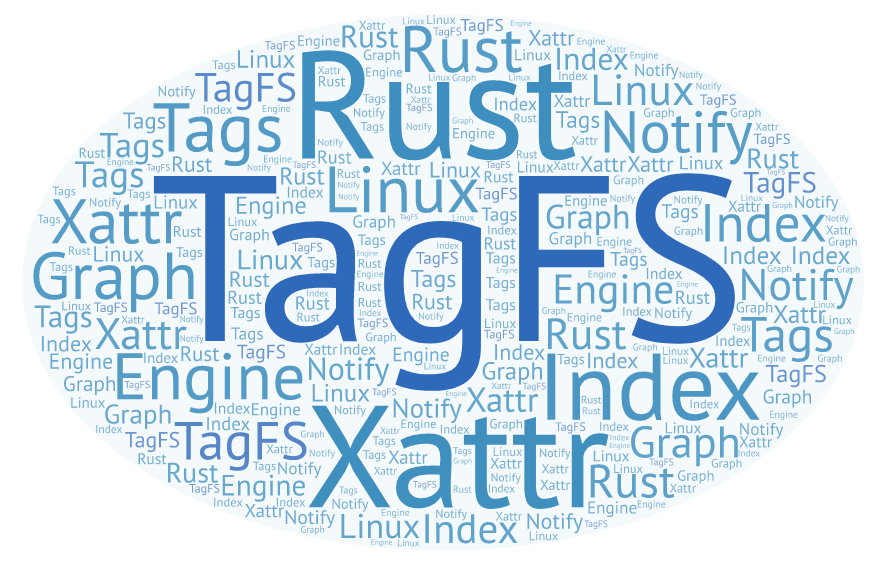
\includegraphics[width=0.43\textwidth]{images/title.png}
% 	\end{center}
% \end{figure}

\begin{figure}[!b]
	\centering
	\begin{minipage}{.4\textwidth}
		\centering
		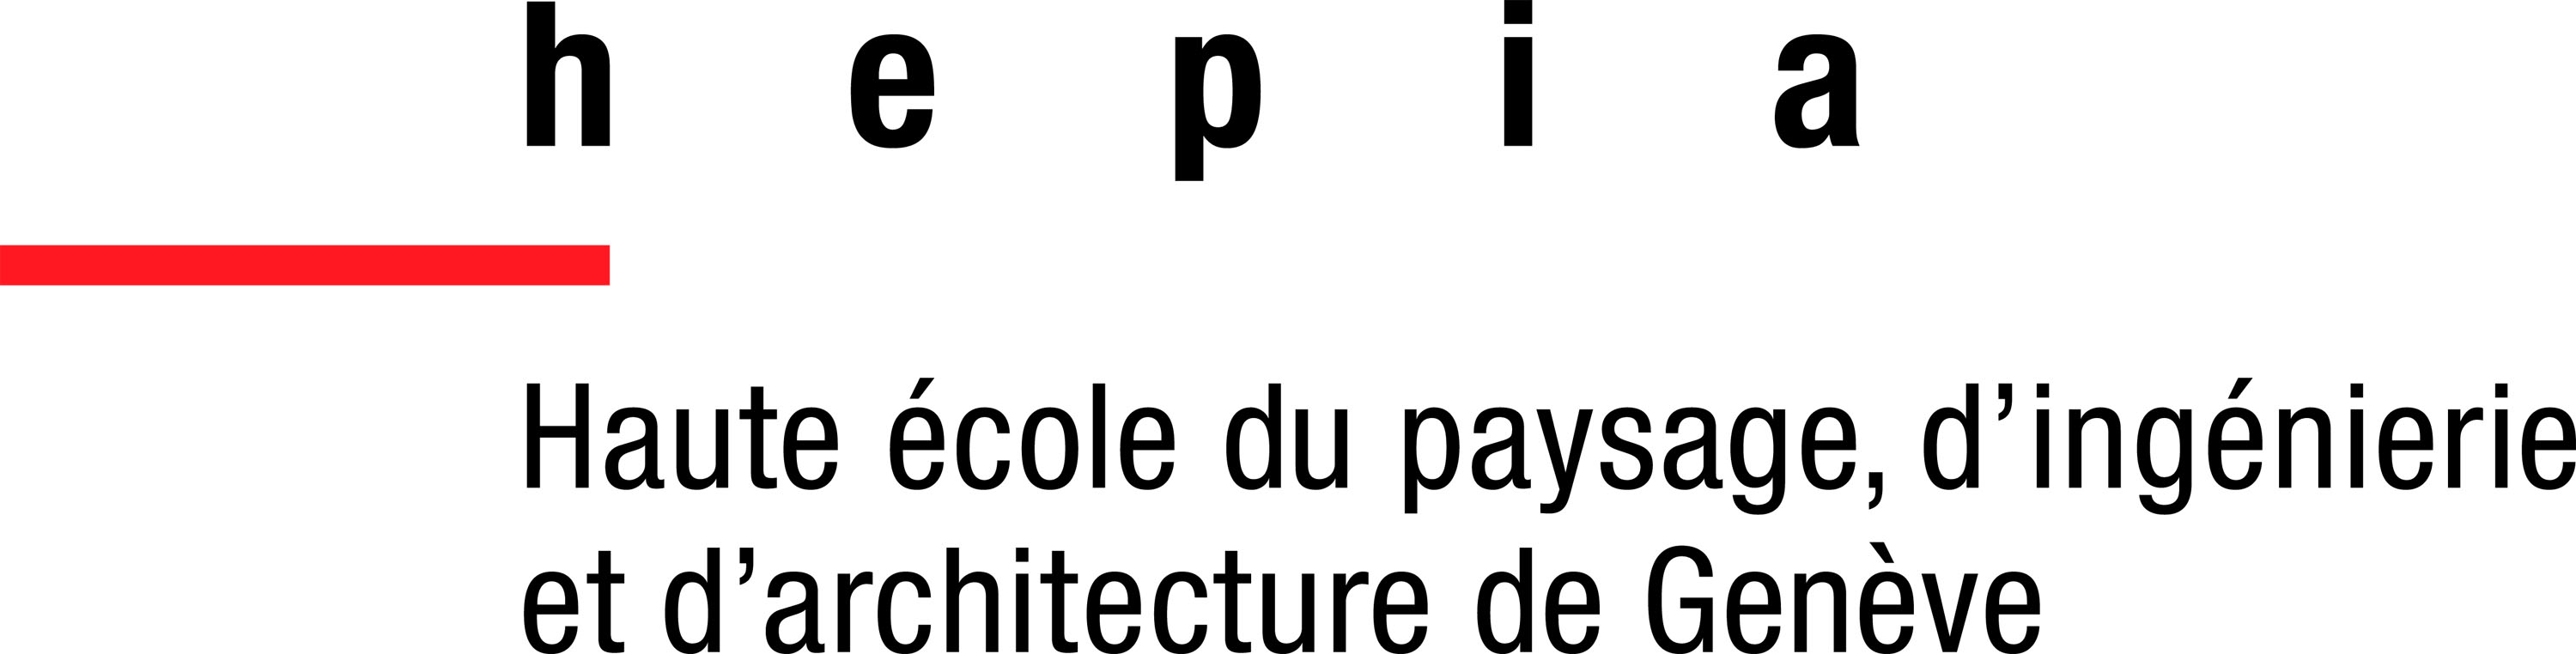
\includegraphics[width=.6\linewidth]{images/hepia.jpg}
	\end{minipage}%
	\begin{minipage}{.4\textwidth}
		\centering
		
\includegraphics[width=.6\linewidth]{images/hesso.jpg}
	\end{minipage}
\end{figure}
\newpage

\newpage

% \setcounter{tocdepth}{2}
\tableofcontents
\listoffigures
\renewcommand\listoflistingscaption{Table des listings de code source}
\listoflistings
\newpage


\section{Introduction} %--------------------------------------------------
\cite{ref0}
\cite{ref1}
\cite{ref2}
\cite{ref3}
\cite{ref4}
\cite{ref5}
\cite{ref6}
\cite{ref7}
\cite{ref8}
\cite{ref9}
\cite{ref10}
\cite{ref11}
\subsection{Motivations}
\subsection{Buts}


\section{Analyse de l'existant} %--------------------------------------------------
Dans cette section, nous allons analyser les principales solutions existantes, qu'elles soient 
intégrées directement dans un système d'exploitation ou sous la forme d'applications utilisateur.

\subsection{Fonctionnalités incluses dans le système d'exploitation}
% \subsubsection{BeOS}
% \subsubsection{Linux}

\subsubsection{macOS}
macOS possède son propre système pour étiqueter des fichiers. Il est intégré depuis la version 
OS X 10.9 Mavericks. Depuis l'explorateur de fichiers, l'utilisateur a la possibilité 
d'ajouter, modifier, supprimer, rechercher des tags. Les fichiers peuvent avoir plusieurs tags 
associés. Un code couleur permet de plus facilement se souvenir et visualiser les tags attribués. 
Dans l'explorateur de fichiers, les tags se retrouvent sur le bas côté, pour y accéder plus 
rapidement. 
\begin{figure}
    \begin{center}
        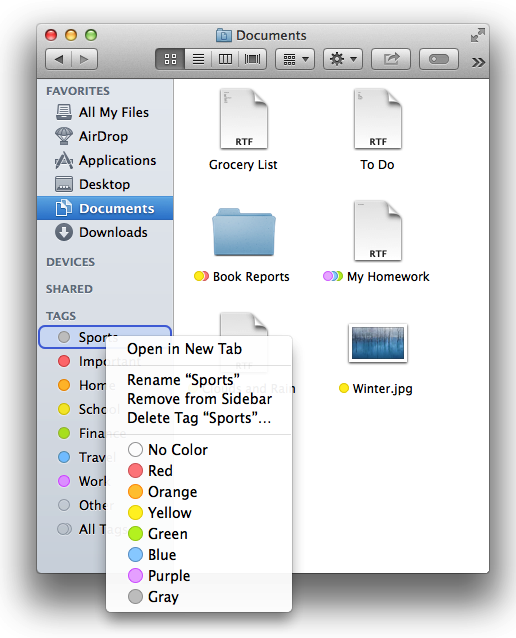
\includegraphics[width=0.7\textwidth]{images/macos_tags.png}
    \end{center}
    \caption{Vue et gestion d'un tag dans le Finder macOS (\cite{ref5})}
    \label{macos_tags}
\end{figure}
Lorsque l'on clique sur un tag, une recherche Spotlight est effectuée. Spotlight est le moteur de 
recherche interne à macOS. Spotlight garde un index des tags, fournissant un accès rapide aux 
fichiers correspondants.
Tous ces tags peuvent se synchroniser sur les différents "iDevices" via iCloud. Finalement, 
un menu de réglages permet la gestion des tags (affichage, suppression, etc.) (\cite{ref5}, 
\cite{ref6}). L'implémentation de ce système utilise les extended attributes (voir section 
\ref{extended_attributes}) pour stocker les tags. Les différents tags se trouvent dans l'attribut 
\mintinline{shell}{kMDItemUserTags}, listés les uns à la suite des autres. Via le Terminal, à 
l'aide de la commande \mintinline{shell}{mdls}, nous pouvons afficher la liste des tags associés à 
un fichier, nommé "Hello" pour l'exemple :
\begin{code}
    \begin{minted}[bgcolor=mygray,breaklines,breaksymbol=,linenos,frame=single,stepnumber=1,tabsize=2]{shell}
% mdls -name kMDItemUserTags Hello 
kMDItemUserTags = (
    Green,
    Red,
    Essential
)
    \end{minted}
    \caption{\mintinline{shell}{mdls} listant les tags d'un fichier sous macOS (\cite{ref7})}
\end{code}
\bigbreak
Ici, ce fichier "Hello" est étiqueté avec trois tags, "Green", "Red" et "Essential". Le fait que 
l'indexation est réalisée avec Spotlight implique une réindexation des fichiers dans le cas d'un 
changement de nom pour un tag donné sous macOS. Le framework système FSEvents donne une solution 
partielle : c'est une API (utilisée également par Spotlight) qui offre aux applications la 
possibilité d'être notifiées si un changement a eu lieu sur un dossier (un événement toutes les 
30 secondes). FSEvents maintient des logs de ces changements dans des fichiers, les applications 
peuvent ainsi retrouver l'historique des changements quand elles le veulent (\cite{ref10}).

\subsubsection{Windows}
À partir de Windows Vista, Microsoft a ajouté la possibilité aux utilisateurs d'ajouter des 
méta-données aux fichiers; parmi ces méta-données se trouvent les tags.

\subsection{Applications utilisateur}
\subsubsection{TagSpaces}
\subsubsection{Tmsu}
\subsubsection{Tagsistant}
\subsubsection{TaggedFrog}
\subsubsection{Tabbles}
\subsubsection{Dropbox}
% \subsubsection{SemFS}
% \subsubsection{Oyepa}
% \subsubsection{dhtfs}
% \subsubsection{tagfs (marook)}

\section{Analyse des besoins} %--------------------------------------------------
% surveillance des fichiers
% indexation



\section{Technologies} %--------------------------------------------------
\subsection{Rust}
\subsection{Les extended attributes}\label{extended_attributes}
\subsubsection{Théorie}
Les extended attributes, ou "attributs étendus" en français, sont un moyen d'attacher des 
méta-données aux fichiers et dossiers sous forme de paires \mintinline{text}{nom:valeur}. Ils sont 
stockés dans les fichiers. De nombreux systèmes de fichiers gèrent leur usage : ext2-3-4, XFS, Btrfs, 
UFS1-2, NTFS, HFS+, ZFS. Dans le cadre de ce projet, l'accent est mis sur ext4. 
\subsubsection{Petites manipulations}
% inclure fichiers text

\subsection{Notifications}



\section{Architecture} %--------------------------------------------------


\section{Réalisation} %--------------------------------------------------



\section{Discussion} %--------------------------------------------------
% cahier des charges rempli ?
% réalisation OK ?
% performances
% Rust VS C
% Bugs
% Améliorations futures



\section{Conclusion} %--------------------------------------------------
\subsection{Remerciements}


\newpage
\section{Références} %--------------------------------------------------
\bibliographystyle{unsrt}
\bibliography{bib}

\end{document}

% \begin{figure}
%     \begin{center}
%         \includegraphics[width=0.8\textwidth]{images/image.png}
%     \end{center}
%     \caption{légende}
%     \label{label}
% \end{figure}

% \begin{code}
%     \begin{minted}[bgcolor=mygray,breaklines,breaksymbol=,linenos,frame=single,stepnumber=1,tabsize=2]{rust}
% fn main() {
%     println!("Hello, world!");
% }
%     \end{minted}
%     \caption{Hello world en Rust}
% \end{code}
% \bigbreak

% \begin{code}
%     \inputminted[bgcolor=mygray,breaklines,breaksymbol=,linenos,frame=single,stepnumber=1,
%         tabsize=2,firstline=157,lastline=185]{rust}{file.rs}
%     \caption{légende}
% \end{code}
% \bigbreak
